\chapter{The Game}
(which you just lost)

Once you pop into the game, you are assaulted by either a weird look of symbols, or a weird look of things barely resembling a crude depiction of the world.

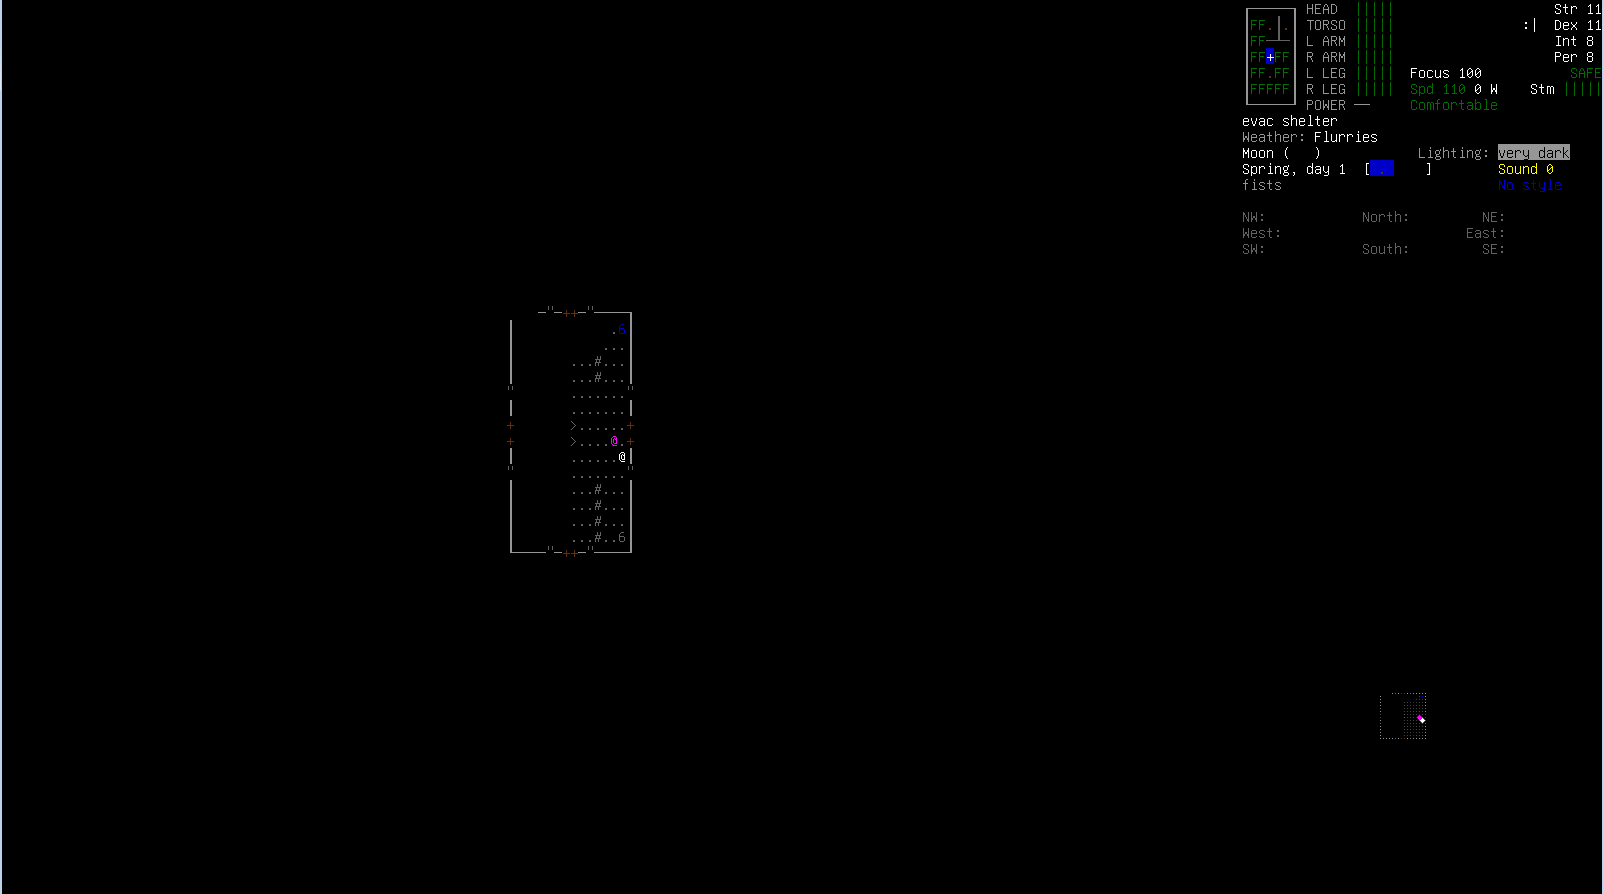
\includegraphics[width=\textwidth]{03}

Woah, who turned off the tileset?

Well, that was me, to give you a general idea of how the game looked in its' original form (which is honestly quite good, especially if you have enough imagination to fill out the blanks, ASCII is something I can always recommend.) if you however press [Esc] to bring up the quick menu, go to Options (or press 2) then cycle to Graphics (lol) using the [TAB] key and scroll down to the "Use Tileset" option, you can and should turn that on. Directly after you can also set up your favorite tileset to be used. I personally use the MSX++LIVE\_PEOPLE Tileset, which is a Fork of MShock, which got forked and improved several times and turned out to be one of the best tilesets so far.

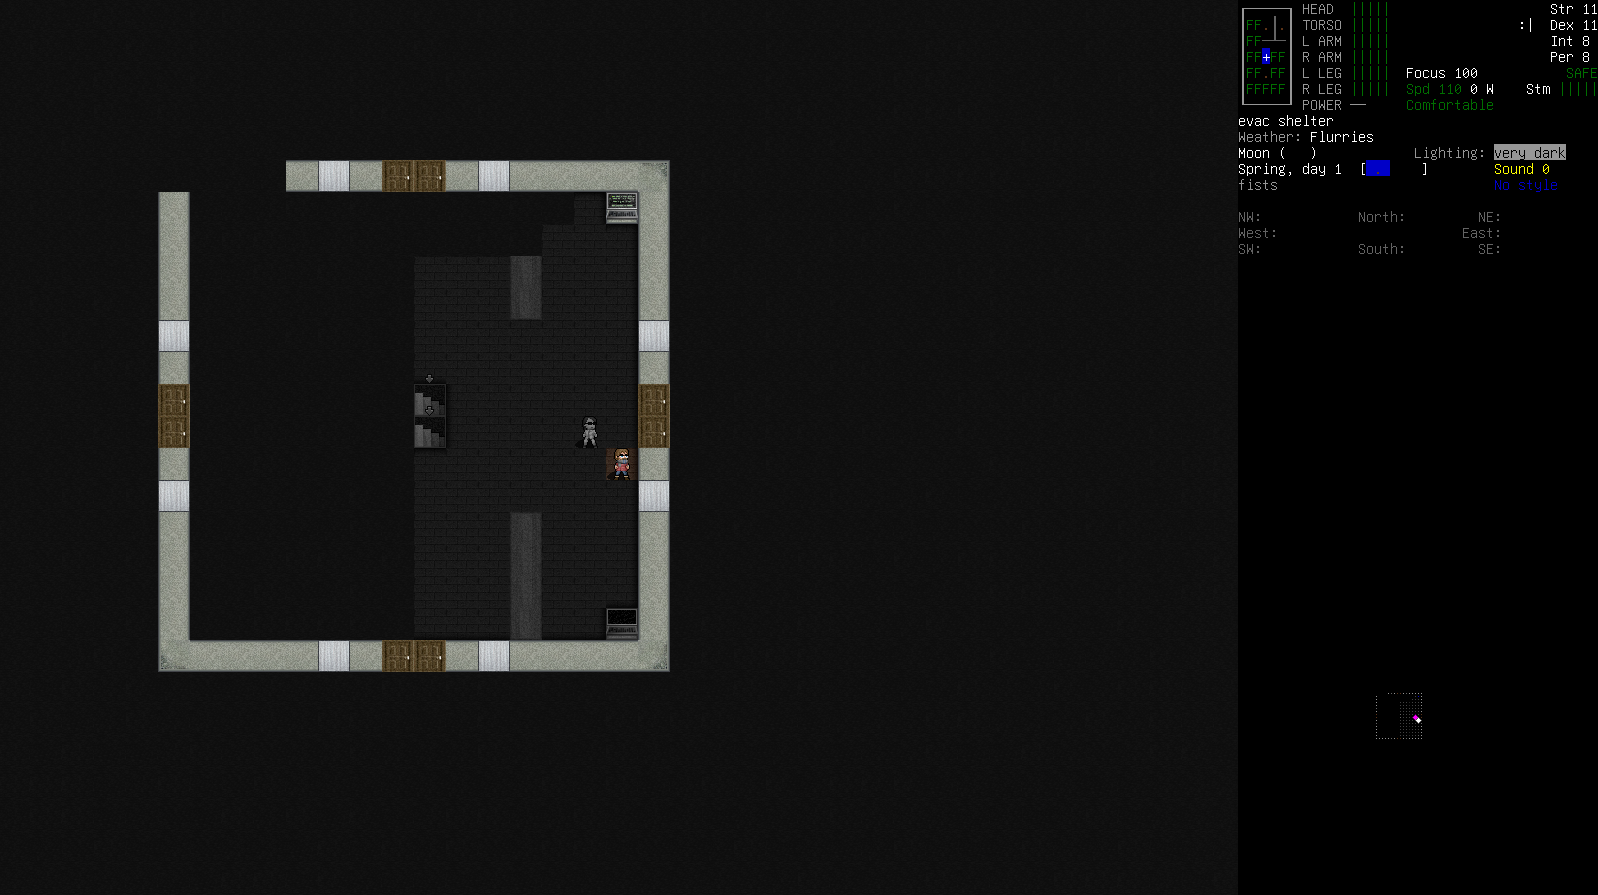
\includegraphics[width=\textwidth]{04}

Ahh, way better, at least you can now determine what's what at a glance. But what's with all that stuff on the left and right side of the game window? The left side might be somewhat self-explanatory, being that you can tell what is located where. On the other hand, the right side seems so cluttered that you are flat-out bombarded with information.

\section{Interface}

(well, that got a rework, but hey, they just moved the stuff around, the contents are still the same)

To get to the Interface that you are now presented with I'm going to use the screenshot again as an example.
The entire left side of the game is your view on the world, what's where, where you are in relation to everything else and so on and so forth, when you issue a command, like a move, this view will slightly change.

On the Right side is the status bar, filled with information that is quite daunting to look at.

At the very top left of it, there is a small 'Overmap Compass', it shows you what the surrounding overmap tiles are, for example roads, forests, houses that come up ahead. Directly below it you can see the name of the tile you are standing upon

To the right of that is your HP, represented as green bars, or if you picked up the Self-aware perk, in numbers.

Wait what? 6 HP Bars to keep track of? Yes, damage done to you in combat is in turn reducing the HP to the attacked body part. This also allows you to see at a glance, what immediate effects your body parts - a red name besides the bar indicates bleeding, blue means a deep wound, green means the body part is infected. If the Health bar changes from numbers to (\~{}\~{}\&\~{}\~{}), it means that the limb is broken and currently not functional.

And directly below is a POWER indicator that only has a bar in it, this is for your current Power to CBMs that are installed into you. As we don't have any CBMs, nothing to see here.

Next up - that empty space in between that and the smiley. Yes, there is something there, you just can't see it. That is where your characters' needs are located. If you feel thirsty, hungry or in dire need of a spot to sleep in, the game will tell you this on that empty spot, even colour coded: yellow means the effect is minor and starts to set in, light red means it is starting to become a real problem and is currently affecting you, dark red means you have a serious issue that could turn out to be lethal in one way or another.

Right below that empty space you see your current amount of focus. This plays an important role in skill gain, but more on that later.

Now for that sweet smiley that looks at you with its' currently more than uninterested look (:|) - this is your general happiness indicator, ranging from (D8 - depressed) all the way to (8D - elated), more on that later when we talk about the mechanics of the game.

On the right of that you can see your Stats, and if they are lowered(red) or boosted(green) by various effects. As we can see, we have 11 Strength, 11 Dexterity, 8 Intelligence, 8 Perception, all things seem to be in order.

Right below the stats you see a fat, green SAFE - this indicates safe mode, a mode that will notify you if something potentially threatening enters your field of view and stopping inputs until you disable it[!] or ignore the monster ['] that caused the alarm. It is a great feature that saved so many players when just doing a walk from A to B without paying much attention, just by enabling safe mode again [!].

Left of that fat green SAFE notifier, you can see some numbers. SPD 110, 0 W and a comfortable in green below that. This gives you an indication of how fast you are. Given our perks, we have a speed of 110\% and since we haven't taken a step, walking speed hasn't changed yet.

Comfortable in the apocalypse? well that is going to change, one way or the other. This is just a general indicator on how the temperature outside feels to you with your current amount of clothing on.

Below the location name are currently positioned is the current weather as well as the moons' position. So we know there's some small snowfall going on, and we can't discern the moon's location. Oh well, could be worse.

Right of that is the indicator for light levels: Lighting: Very Dark, meaning we see jack shit as of right now. Why is that? well, all the curtains are closed. Light plays an important role in noticing things and things noticing you (bare a couple monster differences)

Directly below is a calendar, showing the date as well as the season, with an indicator for the suns' position. Since we don't have a watch yet, we can only tell time by looking at the sky, barely.

The yellow sound: 0 to the right of that is an indicator of how loud things are that happen around us. Whenever you take a step, you produce noise depending on some of the gear you are wearing, traits (light step reduces noise noticeably) and/or CBMs and Mutations. Whenever something else in thesurrounding area happens (buildings collapsing, land mines going off), there will also be a bump on that noise indicator there.

The blue 'No style' statement below is showing you what weapon or martial arts style you are currently using. Since we don't own something as fancy as that, we don't use any particular style.

The Directional Indicators - the REALLY important interface panel for the observant survivor. Whenever a monster enters your field of vision, it will be positioned with its' overworld Symbol and its name in one of these indicators, according to its position towards you, obviously.

The big empty space below all of that is a log for messages. How much damage you do, how much damage the enemy does, if you evade an attack, what you just did, everything remotely thinkable off will land in there. By pressing [P] you can access the message log and scroll through recent messages you may have missed.

And last but not least, at the very bottom is a radar that shows you a more detailed look of what you can see. Enemies would be marked as red dots, NPC's as violet dots and so on and so forth. Makes finding minefields somewhat easy if you know their pattern and o
ccurrence positions.

And that pretty much covers the interface, all of those funny values will change when you play, either to the positive or negative, depending on how you do.

\section{Game mechanics}

As cataclysm is a roguelike, it has some mechanics that are inherently difficult to understand for someone who has never touched a game like this before, but even for veterans of the roguelike genre, some of the extra mechanics provided tend to be a bit difficult to wrap your head around. But to give you a general overview on how things are handled on a base level - The game is basically paused forever, unless you do a move. Whenever you perform an action that takes time, everything else performs an action that takes time. This means movement, using items, combat, while things like inspecting what's around you, checking your inventory and the likes do not take time (for whatever reason, maybe you have a photographic memory). So whenever you move, everything else does. You striking an enemy? So does the enemy. All of this is according to the speed of each entity. You have a base speed of 100. Enemies have a base speed according to their internal values (Zombies are usually slow as shit while some wildlife as fast as a road runner). Everything that happens around you is measured in speed relative to you. If you are being slowed down due to pain, poison or whatever, surrounding entities can perform more actions in the time it took you to perform that one action. This can be a pretty annoying effect. While you struggle to swing a slow weapon at the enemy, he can have already performed several hits to you. Which is why it is important to always check your condition. In the following chapters we will talk about the various possible mechanics that you will come across more in-depth.

\subsection{Your Characters' Needs}

Everyone has needs, you do, I do, so why shouldn't your character in a survival game? This is something that you most likely will struggle with in the early game to keep track of, later on it will be more or less just a regular task on your list to tick off. But first and foremost, you should understand what needs you have, how they work and how they can affect you.

So how do your needs work? Every need has an invisible numeric counter in the background ticking down whenever time passes in the game. Once the number goes below a certain point, you will be notified in that blank space to the right of your health, and your stats may be affected. The more pressing a need is, the heavier the impact on your performance.

The big one and I mean the BIG ONE is water. Water is essential for survival, without water, you are a goner within a couple days at best. While being thirsty in itself is not much of a problem, barely reducing your speed (extremely small \% amounts), it can add up with other negatives, so having a drink every now and then keeps you happy, and more importantly, keeps you alive. Having a good supply of drinkable water is mandatory for any basic form of survival, besides it being the need that ticks down the fastest, which is also why it is your most important need. Beware, as many sources of water are not inherently drinkable. Most notably - toilet water, which newer players tend to drink without checking the consequences. Drinking unpurified water carries the risk of giving you food poisoning. While ponds and rivers have a chance to poison you, it is in a pinch doable to drink from them to quench your thirst, remember that you are taking a risk. And vomiting out the water and potentially food you had beforehand would just waste supplies as well as hitting your mood badly for a while.

The next big thing on the list is food. Food comes in various shapes, tastes and forms, but it all has one important factor - to keep your stomach filled and you running. Being hungry has no negatives at all, but being famished or worse starts to impact your stats and speed. But rejoice, food is plentiful if you know where to look. Forests have edibles in them for most of the year (Note: Food balance changes made forests way less appealing for their veggies, more for their Nuts and wild game) You can get by eating junk food you looted from houses, off of enemies, but sooner or later, you want to properly stock up on long lasting food.

On the note of finding and eating food found in the wilds - do NOT eat unprocessed food unless you absolutely have to. Eating raw meat carries the risk of catching a food parasite, which are not only unlogged in the games events (meaning you will not be notified), but can also severely hinder any progress until removed by drugs. These hindrances are draining food and water supplies quicker, unexpected pain, messages about your joints aching or hallucinations (depending on what type of parasite you caught). Also, raw veggies usually carry a mood penalty to be eaten raw, so while it works in a pinch, the extra mood drain will quickly stack up and slow further progress for a while, you're therefore better off processing them in one way or another.

And that leaves us with sleep. While sleeping is nice to skip the nights in which you can do only so much unless you have a permanent light source (Which, if you spawned in the shelter, you have in the form of a lit-up Terminal) it is also essential to not suffer sleep deprivation. While it is the need that is the least necessary, it still is a necessity, simply because being dead tired imposes a great hit on intelligence (-4) and therefore makes crafting way less efficient. To go to sleep, hit the [\S] button and select that you want to go to sleep. You can sleep anywhere, from the concrete of the road, to a bed or in a vehicles' seat. Each on its own having a certain difficulty to fall asleep on. Sleeping on a hard floor is obviously way more difficult than sleeping on a bed, but even if that is not a possibility, a bench or table is better than sleeping on the floor. There are also items that assist you in falling asleep, like pillows. Just have them on the tile you wish to fall asleep in. Remember though, that you just don't fall asleep the instant you lie down, and being sated and full, having a proper bed (or seat) to sleep in, as well as actually requiring sleep makes it all the easier to fall asleep. Make sure to go to bed early and potentially wake up earlier, as waking up late means you wasted precious sunlight in which you could explore, craft and loot.

While not technically a need, you will quickly perceive it as such: Your happiness, or in other terms - the mood.

Mood is an interesting thing to take notes from: If you are unhappy with life, you definitely will feel the negatives, while being happy seems to have little effect on your day to day life. But how does it actually manifest its' negatives? Well, for once, you will be slower in crafting or straight out refuse to do work (this includes vehicular work and butchering/disassembly), however, your skills will also be affected, though in a different way - you will gain experience much, MUCH slower than normal. How come?

You remember that smiley as well as your Focus points? Those now come back into the talk. Your mood, at a quick glance, is depicted by that smileys expression and colour, red meaning bad, green being good, totally fine so far. Your mood (viewable with [v]) will also list your current focus point gain/loss per minute. Being unhappy drains focus, being happy refills it quicker. But what is focus? In simple terms - it's unspent experience. You spend this experience by performing actions that would gain you experience in a respective skill whilst draining from the pool of focus. So the more focus you have, the better you are off to train skills, either by reading or by doing the actual related tasks.

So what should you aim for on your focus? The higher the better obviously. But, what is the normal value of focus? For any character without any particular mood effects, it tends to fluctuate around 100, depending on actions done. High mood increases this to 130 somewhat easily, with some dedication and work put into it, values of 160+ are achievable. But this can also turn the other way and you can easily end up with being stuck at 30 focus, either by draining it heavily - combat is a great way to do so - or by doing bad things. But what could be considered bad in a world where there's the living dead and extraterrestrial beings roaming the world? Well, your character is still a human, and may think of human life as valuable. Killing other humans can occur a hefty penalty (killed innocent: -100 happiness), as can losing a friend (long-term companions that you recruited using the 'We're friends' talk option, as you will also consider them a friend, just as they do you). This is not the only threat to your happiness, as things that one would have scruples killing, like zombie children, will occur a small, but stacking penalty to your overall happiness. However, the biggest threat that you can encounter in this regard is not the undead, not the humans (those are too rare anyways to be a bother), but rain!

Being wet, which your clothing most likely will not protect you from, will incur a nasty -55 penalty to your happiness and also carries the extra risk of you catching a cold. While it is absurdly easy to remove (use a towel), you can quickly forget that this is an option.

Another interesting 'need' that may or may not pop up is the need for certain addictive substances. If you started as a character that is currently addicted or you consume too many items of an addiction category too quickly, you soon run the risk of becoming an addict.

Addictions are outright bad. Being addicted can, depending on severity and type of addiction, cripple you for several days or weeks. But how do you actually obtain an addiction?

Every player has a value of 0 for each addiction type - Whenever you consume a drug that has an addictive quality to it, it has a chance of increasing that value by 1 (for each type respectively), this chance is based inside the code for each item. Caffeine is way less addicting than Crack obviously. Once you hit a value of 3, you are considered addicted and will start to suffer the effects if you are craving for that particular substance.

So, how do addiction play out? Whenever you feel a craving, you will suffer negative effects. You may either wish to just ignore it, or take the drug again to sate your needs. When you decide to take a drug, remember that it has a chance to increase your addiction value. Doing so, however, will set an internal 'sated' counter to 1200 (800 for addictive personalities), decreasing each 100 time units, or generally speaking each turn, by 1. Once this counter hits 0, or goes into the negative, you will feel the need for said drug again.
Once you reach a sated counter of 0 - addiction level * 100, your addiction level will be reduced (used to be halved, but changes to the system made going cold turkey take quite the bit longer, now it is almost linear). Note that higher levels of addiction will have more severe effects than just starting to become addicted.

But what negatives are there? These are dependant on each addiction respectively, but more often than not, these effects include morale penalties - depending on addiction type around -50 to -250, reduced Stats, induced nausea, giving you pain, having hallucinations or effects like the shakes popping up.

So drugs aren't inherently bad kids. Just make sure to use them appropriately and sparingly, not liberally. Especially now in the apocalypse, in which your best way of obtaining drugs is to either luck out and find them, or make them on your own. Their respective effects may save your life at some point.

\subsection{Temperature and Clothing}

While each topic on its own could deserve an entire in-depth chapter to it, I decided to put them together, as they are closely connected.

First of all, we will talk about temperature. Every location has a temperature depending on the overall outside temperature and it's insulation. Having open windows in a house will decrease the temperature inside, having a fire inside a house will increase it, pretty standard so far. Outside is usually the coldest (bare one specific overworld special) while some tiles generate heat on their own, like fire or lava. Why does this matter? Because temperature has its effects on you. Being cold ,which changes your temperature indicator from a green 'comfortable'(falling) to a light blue 'chilly' or even worse depending on how cold it actually is, has detrimental effects to your speed. The colder you are, the slower you are, and as we talked previously, being slow means everything around you is relatively faster now, being able to catch up, getting in hits more often and so on and so forth. Not only that, but if your body parts get too cold (yes, temperature is checked for each body part), it'll start to slowly take damage, more so if it gets even colder. This can quickly kill any undergeared character who is stranded out in the wild. The other side of the spectrum isn't much better though. Being warm also slows you down, though not nearly as heavily as being cold. Being hot drains more liquid than usual and being close to various heat sources (fire, lava) also can damage your body parts. Dropping into the very hot! temperature range will put you into the famished food requirement via vomiting and therefore can severely cripple you. So being either too hot or too cold can be detrimental to your health. How do you take on cold temperatures then?

Well...

Clothing is the answer.

Clothing has several different 'attributes' as we will call it here, that define their values for Survival as well as their potential usefulness in certain situations. It should be noted that there is little in terms of limitation when it comes to clothes. You can wear as many pieces as you like, but never more than 2 of the same item. So you can totally wear 2 Backpacks, 2 Duffel Bags, 2 Makeshift slings, but never 3 of them at the same time. This limitation does also apply to Helmets and Boots in particular, as you can only wear 1 piece of Headgear and 1 Pair of footwear.
Nevertheless, let's take it from the top, you could say each piece of clothing has the following attributes:
\begin{itemize}
\item Body part(s) it is worn on
\item Warmth provided to that body part
\item \%-Coverage of the body part(s)
\item Layer it is worn on
\item Encumbrance to body part(s)
\item Armor values provided to equipped-on body part(s)
\item Material
\item Additional modifiers
\end{itemize}

So, now to take a look at these attributes.

The body part(s) a piece of clothing is worn on - this is pretty self explanatory. If you wear something that would cover your entire body, say, a suit, it will cover the appropriate parts, namely the torso, arms and legs. A bandana for example will cover your mouth. You get the idea, You can also just check the items details to see what body parts it covers, as well as...

-Every piece of clothing comes with a warmth value to it that it will apply to the body part that it is worn on. If your clothing piece covers multiple body parts this value is applied to each body piece at the full value. On the note of that, most of the clothing follows logical values when it comes to its' material. Fur is, for the amount of material used, warmer than leather, which in turn is warmer than cloth.

The \% coverage of the body parts it is worn on - The effect of which is really important.

The potentially most important effect later down the line is the effect it has on armor values applying. Think of it like this - If you have a piece of clothing that would provide you with 20 CUT and BASH armor, but has 50\% coverage, that basically means that half the attacks have to be calculated against this armor value, while the other half goes past it unhindered. Makes you look at that piece of clothing a bit more carefully right? With all of that in mind, how are you ever gonna survive in your street threads considering they only provide so much warmth and only cover up so much? Well, this is where'

Layers come in handy - each piece of clothing is not only assigned to a body part, but also to a layer it is worn upon.
There are 4 layers (technically 5)on a body part: Close - belted - Normal - Outer - Strapped

To quickly clarify - belted, or rather 'worn around your waist', as it is called in the game, refers to, well, belts and tools that can be worn on belts via loops. Considering tool belts and the likes are therefore unique to the rule of clothing when it comes to their layering, as they can only ever cover one layer, I just wanted to mention it since you hardly come across a reason to wear more than 1 belt, as they only have so many uses.

Without suffering penalties, you can wear 1 piece of clothing on each layer for each body part. What the layers do to you specifically is pretty simple - for warmth, they add up all the warmth values to that body part. So while outside temperatures could be at a rating of -20 (temperature for the character's feelings' sake is measured on a range, while temperature also exists as a proper scaled unit in Fahrenheit or Celsius, right now, the rating matters) for a naked character, having clothing on each layer with a warmth of 10 (and for the sake of simplicity, 100\% coverage) would put you at a +20 rating, which is pretty comfortable. Going over this would be considered warm, hot etc.

On the note of high temperatures it should be stated that there is no way to reduce the ambient temperature. While you might think that this is not that big of a deal, since, hell, when are you ever gonna be close to a fire, remember that in order to reduce the felt temperature, you have to unequip gear and you only wear so much. If you were to stand close to a burning building for example, all the different Fire tiles generate lots of heat. While this seems minor, the effect that this can have on you can be extreme. There are no limits on how cold or hot an area can be, with several fire tiles stuck close to each other, being near a burning building can quickly raise your felt temperature to a point that will endanger your life, as hot temperatures can have just as negative an effect on speed as cold ones, while also damaging your affected body parts. Sooner rather than later you will have the feelings down for how much clothing you require in the appropriate seasons as well as day times. Usually, the more is better, except for the clothings' negatives'

Encumbrance, or how difficult it is to move in your clothing. Again, layering helps, as you are suffering no penalties for wearing 1 piece of clothing for each layer of a body part. Each piece of clothing makes movement more difficult in a certain way, as each body part has a different negative while being encumbered:

Head:
-does currently nothing and only limits what you can wear (to not stack helmet after helmet on your head)

Eyes:
-negative 1 Per while checking traps for each 10 encumberment
-Extra +0.5 throwing dispersion per point of encumbrance
-extra +0.25 ranged dispersion per point of encumbrance

Mouth:
-running costs + (mouth encumberment lvl * 5) increased stamina
-decreases yelling volume

Torso:
-negative 1\% melee to hit per point of encumbrance
-melee swings cost +1 movement point per encumbrance
-negative 0.1 dodge skill per point of encumbrance
-swimming Encumbrance Lvl /10 * (80 - Swimming Skill Lvl * 3)

Arms:
-extra aiming penalty by 2*arm encumberment

Hands:
-extra reloading time: 30*hand encumberment lvl
-throwing dexterity (throwing - hand encumberment lvl)

legs:
-Running cost + (leg encumbrance * 3)
-swimming cost: encumbrance * (50 - Swimming Skill lvl * 2)
-dodge skill: -encumberment/2

Feet:
-running cost + (feet encumbrance Level * 5)

Basically - the more you wear, the less freely you can move, which, in combat, can be pretty hampering. However, clothing does make up for it, we already know that it has warmth, we know it's protecting you, to a degree, but how does that actually work? We'll talk about that now:

Armor values on gear are what is between you and the zombie that is trying to maul you and use your skull as a muesli bowl. Armor is separated into the following damage types: CUT, BASH, ACID, FIRE, ENVIRONMENTAL. The more it has, the better protected the body part is, makes sense right?

Yes and no, again, coverage is king on the matter of BASH and CUT. Since \%-Coverage determines if a hit done to you will be reduced by your respective armor values, or bypassing it in its entirety. This will be checked for each layer that you wear when a body part is attacked. So it may be worthwhile to stack up on as much armor as possible for each body part, right? No, have you not payed attention yet? Armor that is fully covering and has great protective values will most likely encumber you to hell and back, making you nothing short of a sitting duck, ready to be ripped apart. It is a fine balancing line that you need to find for yourself, how many pieces of armor and clothing you require to not be too encumbered whilst also being protected enough to not just straight-up get killed in close combat.

But what about the other values? Well, Acid protection means that you are able to withstand attacks that would be considered corrosive and that will deal relatively quick damage to the hit body part. You will quickly, and potentially painfully learn to avoid these kinds of attacks once you get into actual contact with them while unprotected. But how does it actually work?

Values in the Category for ACID give you a resistance to being affected by hit acidic attacks. To be able to stand in a pool of acid (not that you'd willingly want to), you would require a flat 5 acid protection on your feet and legs to withstand the acid damage from standing inside a field, yet this doesn't make you impervious to standing in the acid field idle, 5 protection only makes you partially immune, though you do take substantially less damage from it.

Your legs? yes, you only have 6 body parts, 4 extremities, a head and the torso that everything is attached to, so feet and hands are considered to be legs and arms respectively.

Now, what about fire? Well, any gear that is flame-resistant (Basically created out of Nomex) will not only douse you quickly if you managed to get set ablaze, but also reduces the damage to the covered body parts substantially, making it possible to survive a trip into fire. Just don't expect to be surviving for extended periods of time.
As a note on certain materials, clothing that is made out of either cloth, leather, fur or wool will catch on fire and take damage until the fire is put out, or the item in question destroyed.

Environmental Protection? Well, this is something special that I feel should be explained more thoroughly. It will basically allow you to potentially ignore certain field-effects and stop you from catching diseases (if you wear enough mouth protection, that is).

Those field effects are (just to name a few): sludge, acid, electricity, gas of various kinds, webs etc.

As you can see - acid is on the list, so you also require environmental protection as well as acid protection to gain potential immunity, tough this would usually be nothing to work towards on the first couple days, it is something to keep in mind later down the line.
So how does it work?
Well, whenever you would happen to be affected by a field-effect, the game checks its' strength against the strength of your environmental protection for the affected body part.

But there's still 2 attributes to name - so let's go over the material that your clothing is made out of: While the material seems to have little implications on how a piece of gear holds up (leather armor can be nearly as good as a kevlar vest, it all depends on how it's made obviously) when faced in combat, it is the defining factor in repairs. You can use your tailoring tool of choice to fix clothing worn or in your inventory, and whatever material it is made out of is required to do repairs. Not only that, but it dictates the tools applicable as well as the skill used. Items that are worn, yet require fabrications to be made, check against the fabrication skill and more often than not (considering most fabricated things are made out of metals or plastic) require different tools, like a welder or soldering iron instead of a needle or sewing kit.

To go into more technical details about material effects - each material has its own values for defence assigned in the games' files. Each piece of clothing has its own material thickness (which you can't see) assigned to it, this in turn assigns how much protection a certain piece of clothing offers. So in general terms, something made out of Kevlar is generally better than something made out of Leather, except for the fact that the clothing thickness could be higher and therefore superior, but it is a general rule of thumb that does apply.

And last but not least, each piece of clothing can have several extra effects, which I'm going to list:
-pockets
-hood
-rain protection
-gas protection
-radiation protection
-electricity protection
-built-in sheath/holster
-tool storage/loops
-durability (not exclusive to clothes, but is still a special)

Well, what do these do?
The built in sheath as well as the tool storage seem obvious - [a]ctivate the piece of clothing to store an item that can fit into it. It still counts towards the tools you are carrying if you do certain tasks, like a sheathed hunting knife still being able to butcher corpses, or a hammer being stored in a toolbelt if you were to deconstruct furniture.

The pockets are self-explanatory in their description, as long as your hands are free (you not wielding a weapon), you will use those to keep your hands warm.

The hood will be used in the same way, as long as you are not wearing headgear (a.k.a your head is unencumbered)

The Protection from rain reduces your overall penalty for being wet for each body part that is covered. So if you were to get gear that completely covers you and had this effect, you wouldn't feel the effects of rain at all.

Gas Protection is pretty much exclusive to suits in their entirety and Masks, like Gas/Filter/ABC/PBM Masks. Those will require cartridges, as whenever they filter harmful materials, their charge will drain by 1. Make sure to prepare them before heading into battle on gas tiles though, as the preparation delay may cause you to inhale gas before it is too late. Don't worry, charges will only by drained while actively protecting you.

Radiation Protection as well is being exclusive to suits, mostly things like Hazard and Clean suits, these will shield you from any outside radiation. However, if a monster attacks you that would carry over a radiation effect, this will bypass the suit (mostly comes from mods)

Electricity Protection also comes from suits, most notably, the Faraday suit, which will protect you from arcs of lightning zapping you as the suit will be grounded. However, this does not apply to zapback by attacking something conductive (like a shocker) with a weapon that will conduct electricity or your bare hands.

\subsection{Crafting}
Time to talk about the single-most important aspect of the game - crafting.
You wouldn't believe how much code is reserved for crafting alone, especially when you consider that you can also pretty much disassemble whatever you think off. But how does it actually work and what benefits do you, as a survivor, have from it?

To take it from the top, it works by opening up the crafting menu [\&] and being again bombarded with recipes, sitting in categories and subcategories and the list goes on and on.. But not to be intimidated by it, all crafting procedures follow the same steps you need to fulfill to be allowed to craft an item:

You require the appropriate tools (some also require charges)
The appropriate components to make said item
Time, obviously, you won't just create an item in the fracture of a second. (most of the time)
And, optionally, light. If you can't see, you can't craft.

First of all, we need to navigate this place though: [TAB] and [Shift] + [TAB] to navigate the top selectors, [<] and [>] to navigate the subcategories and the arrow keys or NumPad inputs to scroll around inside.

If you however want to look for a specific item, you can also open up the search by pressing [f] inside the crafting menu. You will be shown a bunch of search parameters you can look after. This is a godsend, as it quickly allows you to search for items with the appropriate qualities, what something might be a component out of to guess its' value and so on and so forth. If you have a search results page opened, press [r] to clean the results and head back to the standard crafting overview.

As of the recent versions, the crafting window has been given a new Tab - the Recent/favorite items menu. If you see yourself using certain crafting recipes, but are not interested in searching them all the time, you can just quickly mark them as favorite in order for them to appear in this quicklist instead of you having to search for them each time you wish to craft something. The 'recent' subcategory will memorize the last crafts you have done so you can quickly access these recipes there as well.

Should you notice that you are unable to craft a certain item despite you having all the components, make sure to check if all the conditions are met - is it bright enough or are you too sad to perform a craft? The Top right corner will tell you in red what the issue is. Is one of the tools marked in a brown color? That means the Tool property is on an item that is also a component of the craft. You can't just hammer a rock using itself into pebbles, nor can you use one of your two makeshift welders to turn them into a vehicle welding rig - you require an extra tool that provides you with that quality.

But why is it such an important factor in this game? Well, from boiling water to making powerful firearms with their respective ammo or tailoring clothing, everything that is done via the [\&]-menu is considered a craft, and this is how you, for example, also prepare your food and turn it edible. Not only that, but the devs seem to have thought of so many variables that it's mind-boggling. Forget Fallout 4's scrapping system, this is where it's at. You require a flashlight? No problem, a lightstrip or light bulb, some scrap metal, can or similar container along with some copper wire and an amplifier circuit and voil', one flashlight (without batteries though). And if you were to deconstruct it, you will also receive these same items you were using in that craft. So if you accidentally crafted your last power converter into an item you didn't actually intend to craft, or required that for something else, you might be lucky in that you can deconstruct it. Not everything is deconstructable, as this requires a lot of attention to also include in the code, though the devs have made the effort to include deconstruction - recipes to most items in post, where it makes sense obviously. Items can be deconstructed in the following ways.

open up your inventory, select the appropriate item and select the 'Disassemble' option.

if the item is on the floor, move onto that tile and press [B] to open up the butchery menu, items that can be disassembled will have a selection with a capital letter and only their name next to it. If you wish to scrap an item, you can 'cut it up', however, this will most likely not return all the items and instead scrap resources will be gained.

Use the disassembly menu [(] to select items to disassemble quickly from your inventory or the nearby ground (the 8 tiles around you)

What do you gain from that, apart from the satisfaction of creating that item you want? Well, for once, experience in that respective skill. Crafting things that require the skill electronics increases that, crafting fabrication items increases fabrications and so on. However, there's also the other side of the coin - you can fail on a crafting operation, with different severities.

When you craft, each recipe has its' own difficulty, determined by the skills required and if you meet these and your intelligence (which is weighted against this). If the skill required of the recipe ties with your actual skill, there is a small chance of failing either without using materials ('white fail') or with wasting all the materials required ('red fail'). If you don't fulfill the skill requirements for a certain craft, yet are able to do it because you own a book that contains this recipe to use as a reference, or a follower NPC know the recipe and therefore can also provide you with it, this effect is even more drastic and you will most likely fail. If your skill is substantially higher than the required skill for a certain craft, you will also gain no experience (after several crafts, you will receive a notification in the message log about those tasks being trivial)

On the note of crafting and their respective tools - Tools will never be consumed upon a craft unless they are also part of the components required (the bottom list of items), not while failing or succeeding. HOWEVER - red fails will drain charges from your tools (if applicable)

\subsection{Construction}

Construction pretty much works the same way crafting does, for the most part, and is accessed using the [*] button. It will bring up a list in which you can filter and search, by pressing [f]. Each construction has several requirements:

The appropriate tools
The required Materials
The skill required for it
and a space in which you can build it.
Light is interestingly enough not relevant for doing construction works.

But why would you bother constructing things if there's structures all around the world, ready for the taking? Well, walls can be damaged or broken in their entirety, requiring some makeshift fixing or replacing. You might want to board up windows or doors early in your career to limit visibility as well as entry points for zombies (though they can bash through if they run into it or notice you on the other side). Some tools and stations might help you in your craft, most notably the smoking rack for food preservation or a rock forge for smithing items. Or you just want to dig something resembling a moat by digging deep pits around your base to deal damage to incoming zombies, which are more than willing to step into it (this can be used to create trap areas). So there is more than enough applications for doing it, it all comes down to what you want to do and how much you are willing to invest into a certain location.

\subsection{Combat}

The big challenge when it comes to new players - combat, or 'WHY AM I DYING AGAIN ALREADY OH GOD MY ARMS ARE GONE'.

Combat, while simple to perform, can quickly confuse players with its' many factors and quickly leave them dumbfounded and dead when they were so certain that they could beat the enemy. This is why I wish to make an explanation as to what is happening:

Whenever you were to move into a tile where an entity that is either neutral, or hostile is located you will perform an attack towards that target. It will cost you a fixed amount of movement points according to your encumbrance as well as the weapons speed (encumbrance effects are a flat addition to the speed of a weapon).

Once you do issue the command, you will roll with a x-sided die to check against the enemies defences. Here come all your skills into effect - weapon skills, melee skill as well as the to-hit bonus of your weapon, which flat-out adds (or subtracts if it has - to hit) sides to that die. The die the enemy rolls is sided based on their defensive skills as well as their size (citation needed) and if you manage to surpass the enemy roll, you land the hit.

Same goes for the enemy - if his die, which is affected by the internal melee skill the enemy is given- will surpass your defensive roll (which is decided by your dodge skill modified by your equipped gear) he will land a hit on a randomly targeted body part.

But how much damage does he do? Well, each monster in the game is given a certain damage value, determined by dice with the appropriate amount of sides + a flat damage value, a damage type, and an armor penetration value. So lets say a monster could have cutting damage, 0 armor penetration and 6 dice with 6 sides, as well as +10 damage, this would mean at minimum he would deal 16 CUT damage with a hit (10 flat + 6*1 roll) or at best (for him, not you in this case) he could deal 46 CUT damage (10 flat + 6*6 roll).

This end damage value will then have to pass the armor check. If you wear something on the targeted body part that has 20 CUT armor (we ignore BASH for this real quick) and 75\% coverage, this would mean the enemy has a 25\% chance to bypass the armor value and hit for the full amount of the roll. If he would fail the check, however, the damage value would be subtracted by the appropriate armor value.

So for a hit of 16 damage (the minimum) you would take 0 damage in this case('The enemy hits your [body part] but fails to penetrate armor!'), or you could take a nasty hit of 26 damage -if his damage roll had the maximum damage to it- to said body part, which not only reduces your HP, but also induces pain. Quite severe one at that point. The more HP you lose, the more pain builds up, slowing you down, reducing attributes and so on. So it is difficult to swing back from a fight you are losing simply by luck. If you are winning a fight, you will just 'win more' and the enemy usually won't pull out a fancy magic trick to change the tides' more often than not.

Later game enemies can have special attacks that induce status effects or deal tremendous amounts of damage, so be sure you know what fight you are picking.

But what about pain? Well, it's the reason people die. Not loss of HP, but pain usually is what loses you a fair fight. Damage dealt to you has a certain pain buildup that will increase the current felt pain by a certain amount. Pain is long-lasting and without the help of painkillers, will only reduce slowly over time, but what effects does pain have?

Well, the higher your pain, the slower you are - this is the most obvious effect and also the most brutal to deal with. As you may or may not remember - the slower you are, the faster things around you are (relatively speaking), allowing them to get more hits in. Not only that, but pain also reduces your stats, not too badly early on (very small amounts of pain only reduce Int by -1) but quickly adds up so you can lose heavy amounts in all stats, most notably - Str and Dex, at high Pain levels -3 to 4. And as we know, Str and Dex are defining combat stats. This means that your melee-dice will suffer by getting into heavy amounts of pain, which not only reduces your hit-rate already, but worse yet, pain also reduces your hit chance by a certain amount directly ('Your pain distracts you!'). So, the heavier the pain, the more you are fucked. You can counteract this by popping in painkillers (Aspirin, Codeine, Morphine, Tramadol or homebrew stuff like Poppy Painkillers), this however - depending on how strong the stuff is you just threw into your system - can also have negative outcomes when it comes to your stats. Not just that, but painkillers require a time to kick in properly and only reduce pain by so much, and worse yet, they can be addictive. And if you call now - more nasties - you can overdose on Painkillers and die due to asphyxiation (a Painkiller value of [50]+).

Well, that was a bit of a sidetrack, but a noteworthy addition since it is an important part to keep in mind, since pain dictates the flow of combat and how you might want to behave in the next couple of turns. But what about when you attack something? How does your damage calculate?

Each weapon has its own damage type: CUT, BASH or PIERCE (technically that is also cut with a different flag to it) and other factors that all should calculate into if you want to use a weapon or not, but let's not worry about that, as we will just assume you landed a hit. The weapons damage values (which you can see by checking it in the inventory), as well as your Str damage bonus (visible in the [@] screen) will be added together to your melee dice roll(which will increase with more melee skill at high levels)(citation needed here) and determine the damage done to the enemy minus its armor values. Each enemy has a fixed amount of armor for different damage types - CUT and BASH, as those are the only 2 damage types a player can do. PIERCE is a derivative of CUT and checks against this armor type. Bullets and the likes tend to go for CUT damage (except for blunt ammo, like target arrows, or Beanbag rounds which deal BASH, or piercing ammo like Flechette which also comes with heavy armor-piercing values).

Each strike done against an enemy will, however also have the chance of being a critical hit. This has the added benefit of being maximum applicable damage and your chance to land a critical strike increase with the appropriate weapon skill.

But what about that fun little green bar called stamina? Well, each weapon has a fixed stamina cost to swing. Each movement done has a fixed stamina cost - usually not noteworthy, unless you are overburdened, which increases the cost the higher you are over your limit or when your legs/feet are too heavily encumbered, most likely a combination of both - But we will only worry about the swing. Stamina required for a swing is based on the items' weight and volume and therefore speed - swinging a knife is definitely easier than swinging around a 100L wooden barrel. The stamina cost of your swing will also be modified by the current encumbrance to Torso and Arms. so be sure to not be too heavily wrapped up in gear. Why does it matter? Once you run out of stamina, your swings will hit for less and take up lots of time, not to mention the winded effect, which occurs when you drain the entirety of your stamina and need to catch your breath (-4 all Stats). But swinging fast and for little cost also comes at its' own risk - if you deal next to no damage, you are gonna be winded in no time regardless. This is most notable when doing unarmed combat and also the reason why it is a quick and easy way to get hurt. While unarmed combat is great for murdering zombies once you hit a decent level (3 is minimum for most players, 5+ recommended), when just starting out at rank 0, you will most likely hit like a wet noodle and just waste stamina. So even something as simple as stamina management can be a win or loss determining effect in combat.

This however is most of the things that I can cover in the topic of combat, so we should move on.

\subsection{Status Effects}

While being in combat is no fun - or maybe it is, you masochistic survivor - there's more side-variables you need to pay attention to, not just in combat, but in general. Status effects are ailments inflicted upon you because you stepped into a tile that landed a field effect, got hit with an attack that carries over a status effect, or because of you being unlucky and getting hit by a disease (those are also considered status effects). The variety of effects is great and you aren't supposed to learn them all by heart, but it is something to keep in mind, either when gauging to take that fight or not or what to resolve when moving forward.

Status effects trigger certain events with a certain frequency - what does it mean?

Let's assume you inhaled a lungful of smoke. This is the status effect. It will cause you to cough, which costs you stamina and makes noise - this is its event. You will be coughing at a very quick pace - this is obviously the frequency. So now you are having to wait out its effect, sitting there, coughing - draining stamina, and once you are out of stamina, damaging your Torso HP until the status effect wears off.

This is how status effects work, effect - events - frequency. There is a bunch of status effects that one should be aware off, however, if you ever feel like wanting to know how affected you are, press the [@]-button to see the general character overview and switch over to the current effects window. There you can see which effect does what and how often it does it. Beware that some effects, like parasites, are not listed here. Some status effects you should know about are:

Poisoned/Badly Poisoned - not only deals damage and is considered a painkiller, but slows you down drastically

Painkiller/Stimulant overdose - Occurs once the Value for either Painkiller or Stimulant hits [25], impacting your stats heavily.

Bite wound - If you take a hit from a bite attack during combat that manages to penetrate your armor, there is a chance of you receiving a bite wound. This wound will cause pain over the course of its existence and has the chance to turn into an infection that will inevitably kill you later down the line if left untreated. Treat such wounds using antiseptic items (antiseptic liquid/powder, hydrogen peroxide) or if those are not available, throw some Atryupan into your system and hope for the wound not getting infected, or just pray to whatever higher being you believe in that your health stat is strong enough to not turn the wound infected, as each player has a base chance to not carry an infection and the wound clearing itself after a sufficient amount of time.

And if you manage to not do so or get unlucky, you end up with an...

Infection - This is a serious problem that could end your run. You only have 24 hours from the moment the wound turns infected to being treated by using proper Antibiotics. Not just that, but while you are infected, your stats are severely hampered (-2 each, increasing in severity over the course of the infection) And once the infection progresses far enough, you'll randomly pass out, which is the last thing you want in such a situation.

You could also be extremely lucky and hope for an infection to cure itself, however, a freshly spawned survivor with normal health stat has only an all around 10\% chance of surviving the infection, around 25\% if you picked the 'infection resistant' perk.

Adrenaline Rush - Boost to Str, Dex and Per at the cost of Int (-8), constantly regenerate Stamina and speed boost.

Adrenaline Comedown - speed debuff (-10\%) and Stat reduction (-2 each)

Having a Smoke - +1 Int and Per

The Shakes - This is usually a craving effect caused by addiction, but can also happen due to the trait 'Jittery', which is pretty much the opposite of an adrenaline rush - your dexterity will be hampered at random while under stress or under the effect of Stimulants. (-4, also -1 Str)

Radiation [x] - with x representing the number, your radiation level can have no consequences at all, positive benefits or (for the most part) negatives attached to it. Being irradiated with 1 or 2 points is hardly noticeable, with it slowing you down by only a small percentage amount. Yet, hitting radiation levels of 5 and upwards is where it becomes an immediate Problem that requires fixing. At 5+ you will randomly become nauseous, which in turn could lead you throwing up all the tasty potato chips you just downed, turning the positive mood into a hefty negative. Being irradiated at all also damages your health stat (more on that on the next chapter) while also slowing down your healing naturally and at ranks 10 upwards you will start to take damage to your entire body. Not only that, whenever radiation ticks down, there is a chance of it eating a whole lot of radiation ranks at the cost of obtaining a random mutation, the more irradiated you are, the more likely it is, if the radiation itself won't kill you. So what benefits are there, except you may be glowing in the dark soon? Well, specific perks can work great in combination with high ranks of radiation - Most notably Robust Genetics. If you are willing to gain random mutations, this is a cheap way to just mutating without too many negatives, though you will gain mutations of all different kinds, some may be undesirable despite being labeled as 'neutral' or 'positive'. Another great perk is Radiogenic, which slowly heals you while you are under the effect of Radiation. But for the most part, avoid radiation at all costs and if you have to stay in a radiated area, make the trip short, or pop in some potassium iodine.

Hungry, Thirsty and tired are also listed under the general effects window as status effects with their current level of incapacitation to you.

You should make it a constant habit to check your general overview screen [@] after combat or when visiting certain areas to see if anything special is affecting you, but this pretty much covers all there is to some of the more notable status effects, so we shall move on.

\subsection{HP and Health}

Alright, the big thing that takes up a bunch of your interface, as well as being the determining factor of you either biting the bucket or making it past a hostile encounter. Let's talk about HP first. According to your Str value and the base +60 HP each body part has on its' own, you will have a maximum HP value for each of your body parts, usually somewhere around 80-92, besides that, the interface allows you to quickly tell in what condition a limb is: a red name means you are currently bleeding, a blue name means the body part has a bite wound, green means that body part is infected. Or, if the HP bar looks like this (\~{}\~{}\&\~{}\~{}) it means the respective limb is broken and unusable.

Taking damage from various sources will decrease your HP, while sleeping, having some specific perks, or having a treatment applied will restore HP to you. Pretty standard, but how is it determined how much HP you get? This is in turn decided by your health stat, which is usually hidden (exception being the self-aware perk) and has a base value of 0 and can range from -200 to +200. Being positively healthy means you will heal faster, your limbs mend faster and you will have an easier time fighting off diseases, bite wounds and infections. Being in the negative has the opposite effect, you heal slower (or not at all at -200 health), you will catch diseases more often, fighting off bite wounds is gonna be harder and infections will most of the time be lethal (not like they are already). How do you gain health then and not lose it? Well, health always tries to move towards the middle point, 0, so if you are in the positive, you'll lose health by time passing while on the other hand if you are in the negative, it'll slowly gain towards 0. But you can supplement this by eating healthy foods most notably. Foods found in the wild generally have a positive health value attached to them, as do several later cooking recipes that employ multiple components. For a quick boost in health you could also just pop in a gamma-globulin shot randomly found in households or medical buildings. On the other hand, losing health is surprisingly easy - taking damage, being radiated, eating unhealthy food items all reduce your health rather quickly and start to pile up on the effects of you being slower to heal to peak performance. There are also CBMs, positive and negative, that will affect your health stat. A botched installation can install a leaky bionic, which will constantly eat away at your health stat until you bottom out at -200, while the leucocyte breeder CBM will constantly raise it for a small energy cost.

But didn't I mention limbs earlier? Yes, yes I did.

You see, whenever a limb is reduced to 0 HP, it will break. being unusable and therefore hindering you by either slowing you down if it were a leg, or by not allowing the use of two handed weapons if it was an arm. If your head or torso were to break, it's game over - simple as that. Which is why those two bars are the most important to keep track off, but that doesn't mean you shouldn't care about your other 4 HP bars, as a broken leg can and will severely cripple you and leave you vulnerable.

But how do you fix these? By using your crafting. You can craft splints at First Aid: 1 that allow you to mend broken limbs by wearing the splint on the appropriate body part. (If you have trouble getting the side correct, select the piece of clothing worn and press [C] to change sides) If you have done everything correctly, your HP bar will change from that of the broken status (\~{}\~{}\%\~{}\~{}) to a mending bar (=====). This bar will give you a quick overview on how far your limb is in terms of mending. Being healthy or having the fast healer perks speeds this process up considerably, while being unhealthy or having the slow healer perks will slow this process down by a hefty amount. The bar will change depending on what stage of healing the limb is by filling up with (\#) symbols - So a bar looking like this (\#\#\#\#=) is about to be fully healed. But be careful, each attack done to that limb, regardless of penetration, will have a chance to subtract 1 stage of the mending process. Same will happen if you were to remove your splint while in the middle of mending, so be sure to wear it till the HP bar returns proper. Also, while your limbs are broken or on very low HP, you will feel the effects of temperature on this limb a lot more, mostly resulting in you being more cold so be sure to pack some extra clothing. And with this, you pretty much know all there is to health, HP and everything surrounding it.

\subsection{CBMs}

I've talked about it every now and then and it kept cropping up in different topics, so I guess we will have to have that talk now. So what are CBMs - CBM stands for Compact Bionic Module and are basically nothing but augmentations for the everyman that could achieve the cost. Well, that and survive the operation.

To be able to activate any CBM, you require power. This power doesn't come from just plugging yourself into an outlet, you have to have some power storage banks installed. Not only that, you also require a means to generate power to fill those storages somehow, to which there are several methods, though each of them requires a CBM to be installed to work. Besides those, there are two kinds of CBMs that you can have installed - active, and passive ones.

Active CBMs work by opening up your CBM menu [p] and selecting it via button to drain the energy and activate the CBM. They can have all different kinds of effects, from having flamethrowers built into your hands, to a laser from your fingertip up to a toolset that is useable on demand or just some general utility features like blocking vision or sound. There are also very powerful weapons and combat related CBMs that will drastically increase your damage output.

Then there are the passive CBMs, note that all failed installations will also fall into this category. These CBMs will quietly work in the background for you and can have several benefits (or detriments) like improved Stats, extra Armor or effects like glare protection, while faulty CBMs have severe negative effects that can and will mess up your runs and plans. Some power generating CBMs are also passively working in the background.

But how do you install these CBMs and how do you even obtain them? Well, before we answer the installation, we should talk about acquiring them: For once, some high-tech electronic stores could have CBMs lying around, High tech structures like Military Bunkers or Science Labs are also likely to have easy access to those. But what about in the field? Well, shocker zombies (as well as their big cousin, the shocker brute) come with built-in CBMs that you will need to cut out of them using the appropriate tools - namely a tool with fine-cutting quality, the better the quality, the more chance you have to obtain those sweet CBMs. Many knives come with a fine cutting quality of 1, the X-Acto knife even has 2, but the best tool would be a scalpel, with 3 in fine cutting quality. Makes sense, since hey, you'd require a great deal of precision to make fine cuts to remove something like a CBM without carrying over meaty pieces from where you cut it out. But who'd want to put stuff into them they just cut out of an enemy that is technically considered to be the living dead? Apparently, you do, but how?

Well, the answer to that is the AutoDoc. A relatively new machine that is meant to perform surgical precision installation of CBMs into your system. For it to work, you obviously would require a CBM you wish to install, but also something to knock yourself out cold while this AutoDoc does its' thing. This would be an anesthetics. Those are rare medical items usually found directly adjacent to an AutoDoc, yet come with only so many charges. So each installation needs to be weighed carefully - do you really wanna burn that last Anesthetic kit to install a bit of extra power into you? What if the installation fails and I will be horribly disfigured, or worse yet, die? What about the installation process?

Yes, installing something as machinery into your body is not something to take lightly and that can quickly mess up your run as well as murder you. So, how is the chance determined?

Well, your stats play an important role on that matter. Your intelligence helps drastically when installing CBMs, as do your skills. First aid, computers and electronics (in this order) determine your success chance of installing a CBM. There are three different outcomes:

Success

Failure without incident

Failure with one of the following incidents:
    1. failure with a chance of pain
    2. failure with a chance of body damage (possible if fail > 12\%) (damage rolled from 60-82)
    3. failure with a chance of loss of some or all bionics (possible if fail > 20\%)
    4. failure with a chance to install a malfunctioning bionic (possible if fail > 35\%)
    
Regardless of the outcome, the CBM will be used up. But for the event that you did end up with a failed installation and are now having to remove it, the AutoDoc can do that too, provided you still have Anesthetics left. See why you should weigh each installation decision?

Each installation also comes with a certain amount of time the operation takes, based on its' difficulty, with 1 point of difficulty relating to 20 minutes of operation time. Which, for small CBMs like power storages, only equates to 20 minutes, while late game powerhouses can take several hours to be installed. So you should take caution, as you are absolutely unaware of your surroundings and can be subsequently mauled to death in your sleep, though there are worse ways of dying in this game.

As of time of writing, there is no limitation as to how many CBMs a person can fit into him, however, there is a crude outlier planned to limit your CBM capability per body part with each CBM taking up a set amount of slots in each body part. However, as this system is as of right now not implemented, it is only worth noting that the devs are thinking of limiting CBMs to a degree, simply due to their extreme power.

\subsection{Mutations}

While exploring the lands and encountering all kinds of different areas, you at some point will come across mutations, either by finding mutagens/serums on corpses, being too highly irradiated and mutating by yourself or being struck with an attack that will mutate you. So let's talk mutations.

So, you want to mutate, but how do you do this?
There's several approaches to that. First of all, you can use one of the varying kinds of mutagens, which are obtained from crafting or finding them. You will most likely come across mutagen that is simply labeled 'mutagen' without any prefix as to what it will mutate you into. Consider the 'mutagen' item to be a base that provides you with totally random mutations. More refined mutagens require it as a base component for crafting. So you can either mutate with mutagen at random, hoping to get some positive mutations, or go for the more precise approach of consuming the appropriate mutagen-type that you wish to get your hands on.

If this is too boring for you to bother with, you could also just step into highly irradiated areas like craters and wait till you amass a decent amount of radiation (20+). By simply being irradiated, you will have a chance of gaining a random mutation, just like using mutagen.

And if you don't want to be bothered by the constant annoyances that radiation brings, you could just down a nice batch of sewage samples, misshaped fetuses, arms and legs, as those will also mutate you upon consumption.

I also mentioned enemy attacks and this can be a shocking surprise for anybody out there, wondering as to where they obtained that random mutation from. The most notable and common occurrence (despite it still being a rare occurrence from what I can tell) is the mutagenic laser from Zombie Scientists. If they have trouble reaching you, either because they dropped a flask of acid beforehand and therefore trapped themselves for a short amount of time or are simply stuck in the back of a huge zombie group and can't get to you, they might decide to give you a random mutation instead.

For those interested, when you were to obtain a new mutation through either means, what kind of mutation you receive will be a simple matter of chance, being 66\% to obtain any sort of mutation (positive, neutral, negative) and 33\% of obtaining a bad mutation.

On that matter, the trait 'Robust Genetics' changes these chances as follows: You have a 66\% of obtaining any mutation (same as above), but the 33\% of obtaining a bad mutation will be turned into a 33\% of obtaining a good mutation.

Now that we have talked about how to obtain mutations, we might wanna clear up the most pressing question up ahead. What are mutations?
They are pretty much like traits - you either gain a benefit in a certain aspect, or a detriment. These effects range from a simple increase/decrease to your characters Stats, Bonuses to attacks in form of claws, extra limbs or limitations on what you can potentially wear. Some of the mutations you obtain can also have an impact on your food intake requirements or just have general usefulness like night vision. Mutations are categorized into different mutation-paths. Those range from all different kinds of animals all the way to what one would consider an enhanced human being. Each mutation (positive, neutral or negative) is assigned to one or several of these paths. Heavy mutations in one particular path will allow you to obtain high-end mutations of this path at the cost of locking you out of the other mutation paths permanently. You are, however, still able to obtain the pre-threshold mutations of any other path, positive, as well as negative.

But, what about those negative mutations you are bound to obtain while playing around with those ways of mutating yourself, how do you get rid of those? The answer to that is Purifier - By consuming Purifier, you can remove all the mutations you have collected up to this point. Each use of purifier can, at most, remove 4 mutations. Though this amount usually is only reachable for those that are already heavily mutated. Purifier, however does not allow you to purge starting traits of the character (so don't expect to purify those negative HP traits that you selected at the very beginning), as well as it targeting any mutation you obtained at pure random, so you can be pretty unlucky by purifying all the positive mutations that you obtained, only to be stuck with all the negatives.

Something interesting to note is that mutating randomly is not all that random to begin with. The mutations you obtain first open up certain mutation paths that have these mutations in them. The more paths are already opened by the mutations you have, the lower the chance of a random mutation opening up an entirely different mutation path and instead new mutations will be more likely to improve/worsen currently existing mutations or giving you mutations that are from the paths you are currently on. So, in simple terms - Mutations = Random, the more mutations => the less randomness and therefore the more random -> the less random.

As an interesting side note, mutagens are addictive, mutagenic serums even more so, considering they are just mutagens boiled down until only the really strong stuff remains. Hell, even purifier is addictive to some degree, so don't just down a huge batch of medical serum to mutate yourself all at once.

With all of this in mind, listing each and every mutation that exists in the game would be an abhorrent task and would at this stage just confuse you to the point of being unable to follow what I'm trying to convey. Instead, I will hereby provide you with a link to the appropriate Wiki page:

http://cddawiki.chezzo.com/cdda\_wiki/index.php?title=List\_of\_mutations

It should go without saying that mutations are to be used with extreme caution, as they can flip your game choices around heavily, some might outright ruin your run, while others could save you just as much.

\subsection{The Reality Bubble}

A Topic that we still need to talk about and that may be a bit unintuitive to understand for players is the way this game handles its massive amounts of calculation, since each time you move, every entity does so as well, performing several kinds of actions.

Yet the game doesn't slow down to a crawl and runs like a fortress in DF a couple years in (for the most part), this is due to the feature called the Reality Bubble: With the player as the center, the tiles that are loaded are in a range of around 60 tiles in each direction, resulting in a 7x7 (a small bit shorter) of overmap tiles to be constantly loaded at all times. The Reality Bubble moves the same way you do. Everything outside of that Reality Bubble does technically not exist for as long as it is not loaded.

You may be wondering now - how do crops grow, cars lose/gain charge and all the likes nonetheless? Well, the game works around that, as all of those things are affected on the change of relative time since their last load up to when they re-enter the Reality Bubble.

What does it mean to you, the player? First and foremost it means that that you can cause enemies that you feel are too powerful or annoying to deal with to unload from the game, coming back to them once you feel ready, as they basically won't be able to follow you at a certain point. This is really important for enemies that would spread themselves to an absurd degree, for example fungal enemies. Another effect that you will notice, which happens when playing with Experimental Z-Levels is that the reality bubble spans over multiple layers, meaning enemies and allies alike can follow you up and down stairs, which in turn results in your basement no longer being impervious to enemies so you can't just hide in there, re-gaining HP, step out and poke some enemies to repeat till everything is dead. Not only can you trap yourself, but enemies in locations with enough speed to do so.

\subsection{Vehicles}

Well, you managed to get to this point unscathed, survived, foraged food, killed a bunch of zombies and might even managed to clean out a town, but still have to take the draining hike from your base location to town to do some cleanup or carry around loot? That's what vehicles are for. From a simple dragged cart to a mobile fortress outfitted with lasers - the game got you covered with a system that is even more complex at first glance than crafting, but only at first glance.

So, how is this all working out? Well, you can either find a vehicle you like in the open, on roads or near certain buildings, or create one on your own (which is not recommended for anything that is supposed to drive on your first run), however, most vehicles you will find out there that seem to be functional most likely will come with some problems. They either miss some crucial parts, gas, power or their keys. There are so many possible faults to a car, that finding one in pristine condition with its keys is going to be a rarity. However, let's talk about vehicular controls real quick.

Every drivable vehicle has a location where its' controls are. You need to be on that tile and press the control vehicle button [\^] to attempt to drive the car. When active, you have two sets of possible driving controls - cruise control, or manual mode. Cruise control is just that, you set a speed and the car will accelerate and keep that speed until issued another speed value. you increase/decrease this value by pressing [8] or [2] respectively. With the [4] and [6] buttons, you can turn the car by 15' in the relative direction. Pressing [7] or [9] will do both, a 15' turn and speed increase as does [1] and [3] in the decrease. In order to move with a vehicle, you will need to [5] wait a turn your car to move, you only set the speed and move the appropriate amount of tiles according to your vehicles' speed by waiting. With manual mode you will have to constantly speed up the vehicle to the speed value you wish to drive at. Other than that, the controls are still the same.

Each vehicle will however have a safe and top speed value, which is determined by many different factors, like weight, aerodynamics etc. The safe speed is the speed at which you can drive your car without causing any issues. Going over this speed has a chance to cause damage to the engine parts. And the top speed is just that - the maximum speed your car could achieve when pushed to the max. These numbers can be ridiculously high, so don't worry if you see a sports car being able to achieve a top speed of 600 km/h, this is totally normal in C:DDA, and more importantly, you'll most likely never use such speeds.

But what about working on a vehicle? You do have to find a vehicle that is suitable to drive after all. Well, that is where the 'vehicle overview' window comes in handy, when you [e]xamine a vehicle, you will have the option to check its condition, bringing you to a weird looking screen with all different variables on the bottom, names on the right and some depiction of the vehicle in question at the left hand side.

This is the core of the vehicle system and how you will interact with it.
From the vehicle menu you can [i]nstall parts, [r]epair parts, re[f]ill fuel sources, rem[o]ve parts, [s]iphon fluids, [c]hange tires, [m]end any faulty parts, r[e]name the vehicle or assign cre[w] to a seat. (fixed NPC spot they will take)

But how and where do you install these parts? Well, the left hand view that shows you the vehicle can be navigated using the NumPad. Pressing [i] to install a part onto an existing tile of the vehicle will show you a list of what can currently be installed into that location. Pressing [o] will allow you to remove parts from this location respectively. You can also attach a new structure-part to the 4 cardinal sides of an already existing structure-part, this is used to expand vehicles in several ways, mostly to increase its size and therefore what you can fit into it.

So, with that in mind, with me talking about structure parts and the likes, how are vehicles composed in terms of their parts? Each vehicle has several layers to it, just like clothing, but in this case, it determines where the part is sitting in relative height:
    ' Roof
    ' Center
    ' Fuel source
    ' Engine block LO
    ' Structure
    ' Under
    ' Armor
    ' Anywhere/Other

Something to note is that these positions are not connected to each other in the traditional sense, but only block extra parts of the same category to be installed there. You could have a frame with a solar panel on top, which in turn would occupy the 'Structure' location, as well as the 'On Roof' location of that one tile without actually being connected. The Solar panel is technically just floating up there, firmly attached. This is done to prevent you stacking multiple parts into the same tile, like having 20 solar panels stacked onto the same spot, or several boards in the same Center tile. This way you will have to choose what to install where and it potentially blocking out another part you might have wanted there.

But then again, some parts can only be attached if a certain part is attached already. A quick example - A seatbelt can only be attached on the same tile that already occupies a seat. An Alternator can only be installed in a tile that has an engine it can work with. Same mechanics work the other way around - you cannot remove a seat without removing the seat belt first. This will be mentioned a bit later.

So, with that out of the way, how does it work? Well, to be able to do work on a vehicle, you require tools, a lot of them, each according to the part you want to work on:

Bolt Turning / Fine Bolt Turning (Wrench)
Screwdriving (Screwdriver)
Metal Sawing / Fine Metal Sawing (Hacksaw)
Hammer + Nails (for wooden parts)
Welder + Glare Protection 2 (for metal parts)
Lifting Quality (most likely a secondary vehicle with a lift of some kind attached) OR enough Str to lift it yourself
Jacking Quality (A jack that can lift the weight of the vehicle) OR enough Str to Jack the Vehicle in its entirety

Pr0-Tip: Lifting quality has been reworked constantly in its behaviour - As of right now, the tool with lifting quality needs to be within 4 tiles of the part you wish to remove and requires line of sight (LOS) to the tile.

If you were to make a vehicle from scratch, you will also require at least 1 form of 'Frame' in order to initially start the vehicle construction with. For the sake of this being a complete tutorial, we are gonna assume you will create a new vehicle from square 1.

To start the entire process, you will need to open up your construction menu [*] and select 'Start vehicle construction'. If you have multiple frames nearby, you can select which frame to use, afterwards you are asked to name your vehicle.

After this step, the examine screen will show you your freshly made vehicle - except it's lacking all of the components that would classify it as a proper 'vehicle'. So first and foremost, we should expand this. Assuming we'd be working a 3x3 vehicle, something bare-bones, this would mean attaching 8 more frames to that single one that we have sitting there. Structure parts - meaning frames - are required to attach anything else to it, with the exception of rams, which are slapped next to existing structure parts. By either welding or nailing frames together, you now managed to get a 3x3 of framing set up, looking something like this:

\begin{spacing}{0.75}
+++\\
+++\\
+++
\end{spacing}

But what to do with it? The first thing that would make sense is to slap on some wheels for it to be drivable. The amount of wheels is quite expansive - from simple caster wheels up to Armored 32' wide wheels, lots of different wheels can be attached to the frames. If we were to attach them, we should do it in a location that makes sense, the outer layer of the car. Not like we have much space to work with anyways.

You do require your wheels to be in sensible positions, you can't just have the entirety of 4 (or more) wheels close to the front/back of your car. Doing this will make it unstable when driving and cause you to skid around way more often.

This raises the question of what wheels to put on it. The important factor is that your wheels need to have at least 1 axle that is steerable. Certain wheels, like Wooden Cart Wheels and Banded Wooden Cart Wheels come with the [NOSTEERING] flag and therefore can only be used to have static wheels on them. When installing wheels, make sure to see if the 'Wheel-name' (Steerable) is an option to install it, otherwise you will most likely be unable to turn. Usually 17' wheels from any beat down car are sufficient and shall be used for this quick demonstration.
this would make the vehicle look something like this

\vspace{0.5\baselineskip}
\begin{spacing}{0.75}
0+0\\
+++\\
0+0
\end{spacing}
\vspace{0.5\baselineskip}

Well, we are at least getting somewhere. But now we could require something to sit in, driving would be a bit difficult if we had to stand on the tile right? So let's slap on a seat, even out of wood would be fine, into it.

And on this note, I would like to inform you that ingredient parts can transform into different car parts altogether. While requiring a sheet metal for a roof is logical, you could also use that exact sheet metal to install an aisle onto the floor part of the vehicle. A Steel frame is not just a structure part, it can also be made into a trunk, or door. So check which component is required to install a certain part. A wooden seat for example would take a wooden frame.

So, now we start to take up shape, as we look like this:

\vspace{0.5\baselineskip}
\begin{spacing}{0.75}
0+0\\
+\#+\\
0+0
\end{spacing}
\vspace{0.5\baselineskip}

But wait, how are we going to control the vehicle? It's not like it comes with a built-in control. This is the hardest part and can be frustrating as all hell to obtain, as most vehicle controls inside a vehicle are behind a broken security system, which still needs to be removed (4 mech/4 elec). You could technically try [s]mashing out the broken security system, this however also carries the risk of destroying the other parts, namely the controls. But if you do lack the skills and have an abundance of controls, you gotta do what you gotta do.

This would be the only part (if you exclusively used wooden frames) that requires actual welding to install, so a welding tool is gonna be required at some point or another, it only is a matter of how much you are going to use it.

Well, our vehicle didn't change all that much, but now.. well, we can control it, it has wheels, some of them are steerable. Still, we are missing a way of propulsion. So we have to find a suitable engine. Considering the vehicle would be extremely light at this point, only consisting of a couple wheels and frames, any engine would do, from a simple 1.25l inline-engine to a powerful V12. Considering the fuel efficiency and extra skills required to install a big ass engine, you should go smaller instead of bigger, as the only thing improved is acceleration and maximum safe/top speed. But going too fast might cause risks of their own, namely you driving straight into a minefield, tree or any other hazard, and since we did not yet bother installing a seatbelt, this would send you flying, and most likely, end up dead.

To spark the engine, we also require some form of power, so a battery is also required, with sufficient charge to actually get the engine to fire. An alternator would also be nice, this way your battery will receive charge for as long as the engine is running. These parts are relatively easy to come across, so one would have no trouble finding and installing them. So once we move our ass and collect the required parts, namely a small engine, an alternator plus a battery with a sufficient charge, usually around 10-15\% is enough, we go ahead and install them, for now, into the center tile.

This also goes to show how the system of car parts works. As the engine block is considered to be its own location, it can be installed in the spot with our seat no problem. As the alternator is considered to be an extension part for the Engine, this can also be installed on the same spot and the battery is located in the 'fuel source' location, as it sparks the engine. Battery power is considered fuel for engines, electric motors and tool stations inside a car.

Well, the engine is now properly installed, but now we are lacking something else - somewhere to store the fuel this thing runs on. We forgot to grab a tank of some kind, or maybe you figured this out already and decided to grab one of the different kinds of containers that can work as tanks. But yes, you do also require some form of tank to hold the liquid. From a 10L tank (plastic jerrycan), to the standard vehicle tank (60L) or even a wooden barrel (100L), everything goes. If you have enough fabrication skill and the appropriate tool setup, installing a wooden barrel as a tank is just as suitable as welding in any of the other tanks. It comes down to preference in terms of their durability, required resources etc. But in the end, as long as you have a tank, you are set. If you happen to find a gas station, bring some form of liquid container with you and grab some fuel from one of the different pumps. However, if this is not an option, you require a rubber hose (deconstruct a fridge or cooler from a grocery store) as well. This way you can use the [s]iphon fuel command on any other vehicle you come across to fill up your containers with different sorts of liquid.

So now we can technically finish our car by installing said tank and filling it up with the appropriate fuel. As the battery takes up the center space alongside the engine, you won't be able to install the tank in the same tile, as both are considered to be 'Fuel Source' locations. so you can just install it at the very back of it and call it a day and filling it up once installed using the re[f]ill command in the examine window.

Technically, your car would now be functional and you can just board it in the center location, control it [\^] and go nuts. Though there might be some convenience features you wish to add to your car. Maybe some quarter panels (those are technically see-through, but not passable) all around the drivers' seat except for the back would not only make it look nicer but also protect you from animals and zombies that wish to maul you out of your seat? A seat belt for when you inevitably crash into something you did not account for onto the tile where your seat is located? Or how about a roof on all 9 tiles to make sure you are safe from the rain while driving. And what about that back tile? Well, you could use a wooden frame to install a box in there to store precious loot that you snagged while inside a town.
Well, if we were to go the extra mile, our car may look something along the lines of this:

\vspace{0.5\baselineskip}
\begin{spacing}{0.75}
┌─┐\\
│\#│\\
└=┘
\end{spacing}
\vspace{0.5\baselineskip}


This was more or less just a base tutorial on vehicles to help you navigating the menus, getting the basic idea on how to install parts and what to do with them while not touching on the more complicated aspects like aerodynamics, friction and off road capabilities, those, we will touch now.

Just because you created a block of parts that can basically be called a car, doesn't mean it is as efficient as it could be. Though this design in itself is pretty okay for a start, remember that the bigger your vehicles becomes, the more you want to worry about things like aerodynamics or its' off road capabilities. Why? Because roads can lead to a dead end, or sometimes you have to move off the road to get past a certain roadblock or minefield. Aerodynamics pretty much is a measurement for how fast your car with its current weight and engine power can go and how quickly it can accelerate to the desired speed. How does the value change? Well, most notably, by the cars dimensions. A car with 3 width and 5 length is gonna be way more aerodynamic than a car with 5 width and 5 length (not accounting weight). And you might even be wondering - so what does it matter, can it be that important? Actually, yes it can. Not only does a low aerodynamics value trash your acceleration, which can save you if you need to leg it, but it also inherently trashes the top safe/maximum speed as well as the fuel consumption. The worst part of it is, it doesn't even need to be a full row of structure parts to be considered 1 width more. Something as simple as a wing mirror (which you most likely have seen attached to cars) will already raise the vehicles dimension by 1 point respectively. Instead, if you really need to, install an inboard mirror onto the side windshields that you may have installed in your car. And what about off roading? Well, it is determined by your cars weight against the amount of tire surface. So not only do the wheels diameter play an important role on this matter, but also the amount of wheels. While you can have only so many axles installed to steer, you can slap on wheels that are non-steerable no problem.

Having a better off road value will decrease the chance of you skidding the car around as well as you improving the odds of recovering from said skid, however it also comes at the cost of you requiring more fuel.
With all of this now covered, can we even win this absurd game?

\section{Winning C:DDA}

Simply put - you don't.

There is no such thing as a final goal post to reach, some internal way of telling if you have won or not, no funky easter egg telling you you did it or something along those lines.

It's only you, and you alone. You win, when you declare for yourself that you win, whenever that may be. However, you will most definitely lose, over and over again. Either due to a dumb mistake, some threat you did not yet know existed, or because you were underprepared for the task up ahead, which is the entire reason of me writing this piece. You need to remember that this game is as difficult as you make it to be. The world settings are meant to be tweaked until you find a spot that you feel comfortable in, only to change them later to step out of your comfort zone and tackle new challenges. The professions and scenarios screen provides you with more than enough potential starts that you can test out in order to find something new. And if all else fails, do a random character and see how far you can go with an absolutely unbalanced character that is doomed from the start, only to see how far you can actually take this 'doomed run' from the start and see yourself mutating to become a demigod. It's all up to you, and you yourself are your own worst enemy in this game.

And with this in mind - go ahead and enjoy the challenges you may wish to set out for yourself.